\documentclass[11pt]{beamer}
\usetheme{Bergen}
\usepackage[utf8]{inputenc}
\usepackage{amsmath}
\usepackage{amsfonts}
\usepackage{amssymb}
\usepackage{graphicx}
\author{José Antonio García Hernández}
\title{La susceptibilidad topológica en QCD}
%\setbeamercovered{transparent} 
%\setbeamertemplate{navigation symbols}{} 
%\logo{} 
%\institute{} 
\date{5 de diciembre, 2026} 
%\subject{} 
\begin{document}

\begin{frame}
\titlepage
\end{frame}

%\begin{frame}
%\tableofcontents
%\end{frame}

\begin{frame}{Introducción}
$\psi_x$: campo fermiónico

$U_{x,\mu}$: campo de norma

$U_{x,\mu\nu} = U_{x,\mu}U_{x+\hat{\mu},\nu}U_{x+\hat{\nu},\mu}^{\dagger}U_{x,\nu}^{\dagger}$: plaqueta

\centering
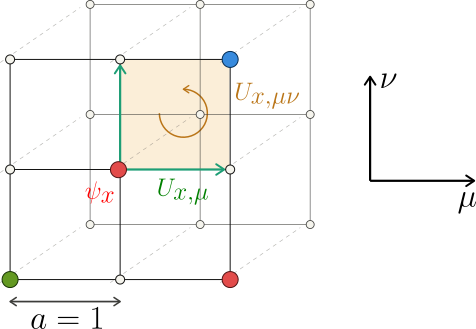
\includegraphics[scale=0.5]{lqcd.png}
\end{frame}

\begin{frame}{Topología de SU(3)}
Consideremos la corriente axial en QCD
$$j^5_{\mu}(x) = \sum_{f}\bar{q}^{f}(x)\gamma_{\mu}\gamma_{5}q^f(x)$$
donde $q^f$ es el campo de quarks de sabor $f\in\{u,d,s,c,b,t\}$. \\~

El lagrangiano de la QCD con quarks sin masa es invariante ante transformaciones U(1)$_A$ y por tanto $j^5_{\mu}(x)$ se conserva al nivel clásico.\\~


\end{frame}

\begin{frame}
Sin embargo, está rota a nivel cuántico por la anomalía de \textit{Adler-Bell-Jackiw}
$$\left\langle\partial_{\mu}j_{\mu}^5(x)\right\rangle = 2N_fP(x),$$
donde $N_f$ es el numero de sabores de quarks y 
$$ P(x) = -\frac{1}{32\pi^2}\epsilon_{\mu\nu\rho\sigma}\text{Tr}\left[ G_{\mu\nu}(x)G_{\mu\nu}(x)\right]$$
es la densidad de Chern-Pontryagin del campo gluónico.
\end{frame}

\begin{frame}{Corriente de número bariónico}
El langrangiano también tiene una simetría U(1)$_B$ relacionada a la conservación del número bariónico, por lo que la corriente
$$j^B_{\mu}(x) = \sum_{f}\bar{q}^{f}(x)\gamma_{\mu}q^f(x)$$
también es conservada. A nivel cuántico se rompe explícitamente
$$\left\langle\partial_{\mu}j_{\mu}^B(x)\right\rangle = N_gP(x),$$
donde $N_g$ es el número de generaciones de fermiones.
\end{frame}

\begin{frame}{El flujo gradiente de Wilson}
Las simulaciones en la retícula estan dominadas por configuraciones que no son suaves. \\~ 

No es directamente aplicable la definición discretizada de la carga topológica por medio de la densidad de Chern-Pontryagin.\\~

Esto causa que la carga topológica $Q$ no sea un entero.
\end{frame}

\begin{frame}
En el continuo, suavizamos la configuración por medio del flujo de Yang-Mills definido por las ecuaciones 
$$ \frac{dB_{\mu}}{dt} = D_{\nu}G_{\mu\nu}, \ \ \ \left.B_{\mu}\right|_{t = 0} = A_{\mu},$$
$$G_{\mu\nu} = \partial_{\mu}B_{\nu} - \partial_{\nu}B_{\mu} + [B_{\mu},B_{\nu}], \ \ \ D_{\mu} = \partial_{\mu} + [B_{\mu},\cdot], $$
donde $t$ es el parámetro del flujo, con dimensiones [masa]$^{-2}$, y $A_{\mu}$ es el campo de norma original. \\~



Se puede demostrar que el flujo promedia al campo de norma sobre una esfera de radio $\sqrt{8t}$.
\end{frame}

\begin{frame}
La versión de la retícula es
$$\frac{d}{dt}V_{x,\mu}(t) = Z(V_{x,\mu}(t))V_{x,\mu}(t) , \ \ \  \left. {V_{x,\mu}(t)}\right|_{t = 0} = U_{x,\mu} $$
con
$$Z(U_{x,\mu}) = -\{U_{x,\mu}\Sigma_{x,\mu}^{\dagger}\}_{\text{TA}}$$
donde hemos tomado la parte anti hermitiana sin traza.
\end{frame}

\begin{frame}
El flujo gradiente puede ser utilizado para fijar una escala física.

Consideremos la densidad de energía
$$ E_x(t) = \frac{1}{4}G_{x,\mu\nu}^{a}(t)G_{x,\mu\nu}^{a}(t).$$

Definimos una cantidad adimensional
$$ \mathcal{E}(t) = t^2\langle E_x(t)\rangle,$$
la escala $t_0$ está definida como
$$ \left.\mathcal{E}(t)\right|_{t=t_0} = 0.3.$$
\end{frame}

\begin{frame}
    En las simulaciones de la retícula medimos $t_0/a^2$
\end{frame}

\begin{frame}{El método \textit{slab}}
Asumimos simetría de paridad que implica que $\langle Q \rangle = 0$.\\~

La carga topológica obedece una distribución de probabilidad gaussiana
$$ p(Q) \propto \exp\left(-\frac{Q^2}{2\chi_tV}\right), \ \ \ \chi_t = \frac{\langle Q^2 \rangle}{V}.$$

Dividimos a la retícula en rebanadas (\textit{slabs}) de volumen $xV$ y $(1-x)V$ donde $x\in[0,1]$. \\~

Denotamos a la carga topológica del subvolumen $xV$ como $q(x)$.
\end{frame}

\begin{frame}
A carga $Q$ fija la probabilidad de tener carga $q(x)$ en la primera rebanada y carga $Q-q(x)$ en la segunda es 
$$ p(q)p(Q-q) \propto  \left( -\frac{q'^2}{2\chi_t Vx(1-x)}\right),$$
donde $q' = q-Qx$.

Concluimos que $q'$ sigue una distribución gaussiana con 
    $$\langle q' \rangle = 0,$$
    $$ \sigma^2_{q'} = \langle q'^2 \rangle - \langle q' \rangle^2 = \langle q^2 \rangle - Q^2x^2 =\chi_t V x(1-x).$$
Como esto es válido para cualquier sector, también es válido con el promedio
$$\langle q^2 - Q^2x^2\rangle =\chi_t V x(1-x).$$
\end{frame}

\begin{frame}{$\chi_t$ en QCD con dos sabores}
\centering
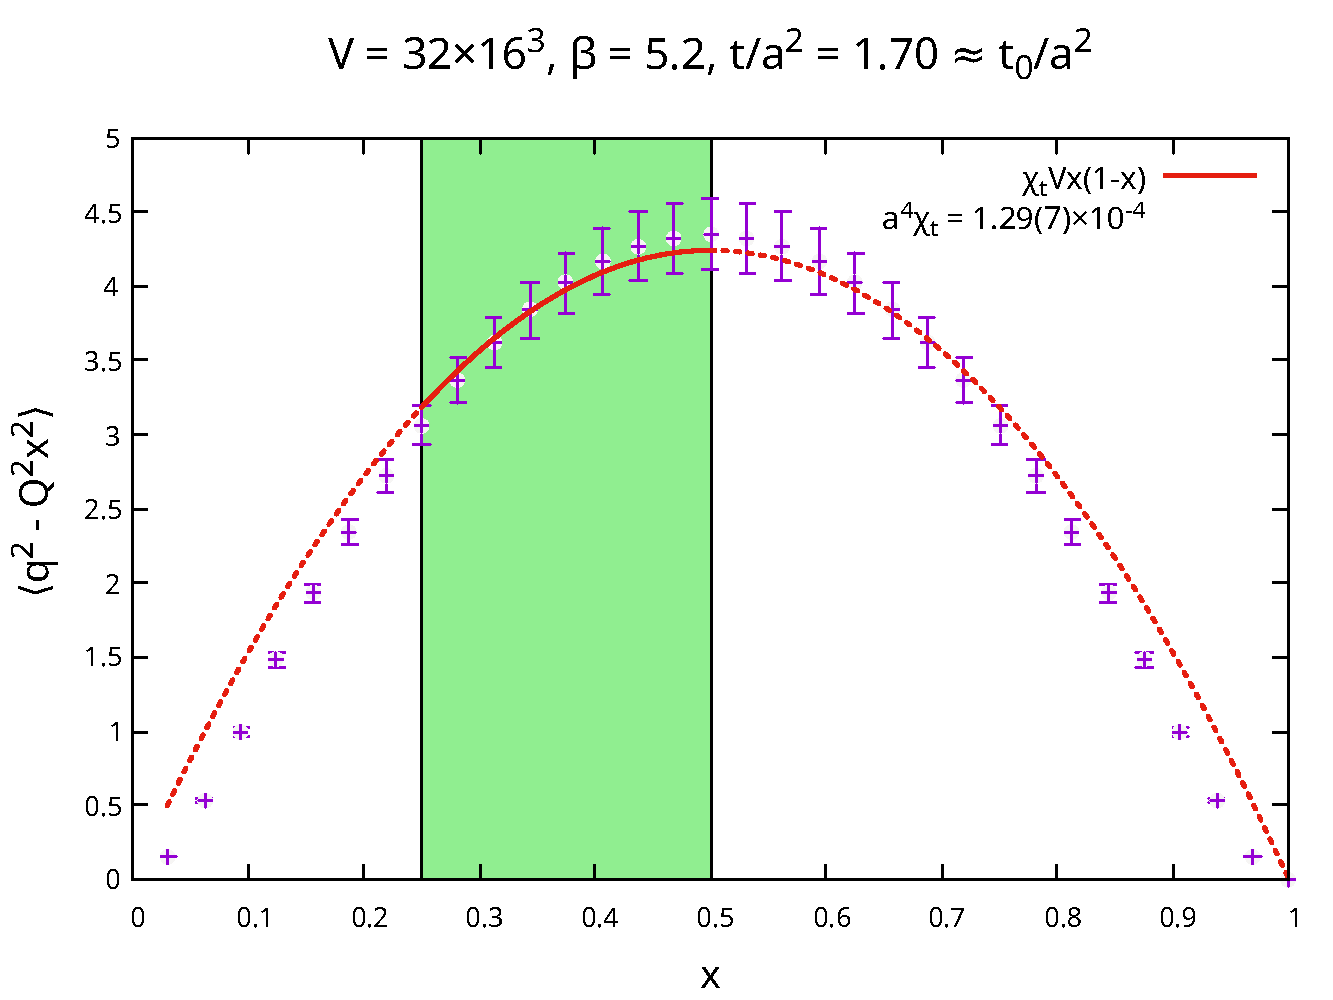
\includegraphics[scale=0.4]{slab.pdf}
\end{frame}

\end{document}
